
	\begin{enumerate}
		\item Дата собрания: 24.10.14
		\item Цель:
		\begin{itemize}
			\item Установить одно опорное колесо вместо двух, чтобы избежать проскальзывания колёс
			\item Попробовать мебельные стяжки в качестве креплений балочных элементов подъемника
			\item Проверить подвижность робота, способность заезда на пандус разворота на нём
		\end{itemize}			
		\item Результаты:
		\begin{itemize}
			\item Приводные колеса робота были отодвинуты назад примерно на 5см, так как робот очень часто вставал на задние колеса и переворачивался при резком старте с места. Скорее всего связано с тем, что основная масса сконцентрирована около ведущих колёс
			\item Стяжки хорошо проявили себя в качестве креплений: они не создают почти никакого трения, при этом сохраняя стабильность конструкции
			\item Робот оказался довольно подвижным, забирается на пандус, разворачивается на нем и спускается без проблем
			\item Программа была написана для максимально легкого управления
		\end{itemize}
		\item Идеи и планы:
		\begin{itemize}
			\item В связи с тем, что работа над колёсной базой почти закончена, мы решили сконцентрировать внимание на подъёмнике, так как это не менее важный узел робота.
		\end{itemize}
				\includegraphics[width=55mm,height=55mm]{Days/24.10.14/9_1_robot}
				\includegraphics[width=55mm,height=55mm]{Days/24.10.14/10_2_robot}
				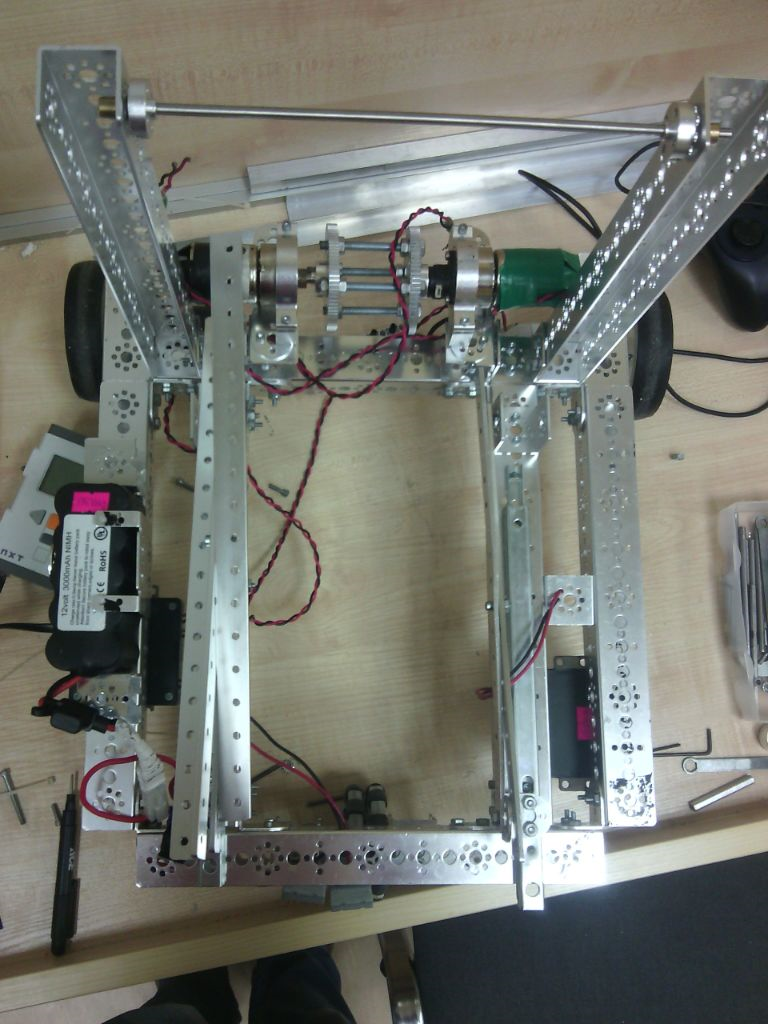
\includegraphics[width=55mm,height=55mm]{Days/24.10.14/9_4_robot}\\
	\emph{Рисунки 11,12 и 13}
	\end{enumerate}
\fillpage
